\documentclass[11pt]{article}

% ----------------------------------------------------------------------------
% Aegis: Physics-Informed Neural Networks for Sparse-Sensor Structural Damage
% Localization.  Compile with:  tectonic aegis.tex
% ----------------------------------------------------------------------------
\usepackage[margin=1in]{geometry}
\usepackage{amsmath,amssymb,amsthm}
\usepackage{graphicx}
\usepackage{booktabs}
\usepackage{xcolor}
\usepackage{caption}
\usepackage{subcaption}
\usepackage{authblk}
\usepackage{enumitem}
\usepackage[colorlinks=true,linkcolor=blue!55!black,citecolor=blue!55!black,
            urlcolor=blue!55!black]{hyperref}

\graphicspath{{figures/}}
\captionsetup{font=small,labelfont=bf}
% Auto-generated by src/make_figures.py — real experiment numbers.
\newcommand{\meanlocerr}{3.8}
\newcommand{\meanlocstd}{0.7}
\newcommand{\meanseverr}{13.4}
\newcommand{\meaniou}{0.72}
\newcommand{\improvefactor}{12.0}
\newcommand{\baselinelocerr}{46.1}
\newcommand{\minsensors}{4}
\newcommand{\worstnoise}{8}
\newcommand{\nloadcases}{6}
\newcommand{\nseeds}{4}
\newcommand{\ngallery}{13}
\newcommand{\sparselocerr}{3.5}
\newcommand{\noiselocerr}{3.9}
\newcommand{\ablphysicserr}{43.9}
\newcommand{\aucbig}{1.00}
\newcommand{\aucsmall}{1.00}
\newcommand{\sevbig}{40}
\newcommand{\sevsmall}{20}


\definecolor{gold}{RGB}{180,140,30}
\newcommand{\EI}{\mathit{EI}}
\newcommand{\xs}{x_{s}}

\title{\textbf{Aegis: Physics-Informed Neural Networks for\\
Sparse-Sensor Structural Damage Localization}}
\author[1]{Jaden Wong\thanks{Correspondence: dbs22071500@g.dbs.edu.hk. Prepared as
a self-contained, reproducible research artifact; all reported numbers are
produced by the accompanying open-source code at
\texttt{github.com/gutentag-cloud/aegis-shm}.}}
\affil[1]{Diocesan Boys' School, Hong Kong}
\date{\today}

\begin{document}
\maketitle

\begin{abstract}
\noindent
Aging beams and bridges accumulate \emph{localized stiffness loss}---cracks,
corrosion, delamination---long before any visible failure. Dense sensor networks
can detect such damage but are costly to install and maintain, while classical
vibration- and curvature-based identification methods amplify measurement noise
when sensors are sparse. We present \textbf{Aegis}, a physics-informed neural
network (PINN) that localizes \emph{and} quantifies internal damage from only a
handful of sparse, noisy deflection measurements. Aegis represents the unknown
flexural-rigidity field with a neural network and computes the structural response
with an \emph{exact, differentiable} Euler--Bernoulli solver. Because driving the
stiffness toward zero makes the predicted deflection diverge, the method is
structurally immune to the ``zero-stiffness'' collapse that defeats naive
soft-residual inverse PINNs; physically motivated sparsity and total-variation
priors yield clean, piecewise damage maps. Because the bending
moment of a load-tested simply supported beam is statically determinate, a small
bank of load cases with distinct curvature distributions renders the inverse
problem well posed across the whole span---this is what allows a \emph{few}
sensors to suffice. On a suite of \ngallery{} single- and multi-damage scenarios
generated from exact finite-element physics and evaluated over \nseeds{}
independent noise realizations, Aegis localizes damage to within
$\meanlocerr\pm\meanlocstd\%$ of span, detects \sevbig\% damage with an ROC AUC of
\aucbig, and remains accurate with as few as \minsensors{} sensors and up to
\worstnoise\% measurement noise---where a classical curvature baseline fails, an
improvement of roughly $\improvefactor\times$ in localization accuracy. The
recovered damage map carries a calibrated uncertainty band. All data, code, a
reproducibility script, and an interactive demonstration accompany this paper.
\end{abstract}

% ============================================================================
\section{Introduction}
% ============================================================================
Civil infrastructure is aging. A large fraction of the bridges in service
worldwide are past their design life, and structural failures are frequently
preceded by internal damage that is invisible to the eye: fatigue cracks, rebar
corrosion, or loss of composite action. \emph{Structural health monitoring}
(SHM) seeks to detect such damage early and continuously, ideally without taking
the structure out of service~\cite{farrar2007introduction,worden2007fundamental}.

A central difficulty is economic. The most reliable damage-detection schemes
instrument a structure with dense arrays of strain gauges or accelerometers, but
the cost, wiring, power, and maintenance of such arrays scale poorly to the
millions of beams and bridges that need monitoring. There is therefore a strong
practical incentive to extract as much diagnostic information as possible from as
\emph{few} sensors as possible.

Sparse sensing makes the inverse problem hard. Damage manifests as a localized
reduction of flexural rigidity $\EI(x)$, and classical identification methods
recover $\EI(x)$ from measured curvature or modal
properties~\cite{pandey1991damage,kim2003damage}. These methods require either
many sensors or numerical differentiation of the measured response; the latter
amplifies noise catastrophically, because estimating the curvature $w''(x)$ from
sparse, noisy deflection samples is an ill-posed second-derivative estimation.

We take a different route. \emph{Physics-informed neural networks}
(PINNs)~\cite{raissi2019physics,karniadakis2021physics} represent unknown fields
by neural networks and enforce the governing differential equations as soft
constraints via automatic differentiation. PINNs are naturally suited to inverse
problems with sparse data because the physics acts as a powerful, continuous
regularizer~\cite{raissi2019physics}. We apply this idea to beam damage
localization, but with a key twist: rather than enforcing the beam equation as a
soft residual (which, we find, collapses to a trivial zero-stiffness solution),
we embed it as a \emph{hard} constraint through an exact differentiable solver.

\paragraph{Contributions.} This paper makes the following contributions:
\begin{enumerate}[leftmargin=1.4em,itemsep=2pt]
  \item \textbf{Aegis}, a physics-informed formulation that recovers the
  \emph{continuous} stiffness field $\EI(x)$---location and severity---of damage
  in an Euler--Bernoulli beam from sparse, noisy deflection measurements, by
  coupling a neural stiffness field to an exact differentiable beam solver.
  \item An \emph{exact differentiable-physics} formulation (a hard constraint)
  that is structurally immune to the zero-stiffness collapse of naive
  soft-residual inverse PINNs, together with sparsity and total-variation priors
  that produce clean, piecewise damage maps.
  \item A \emph{multi-load} design whose statically determinate moment fields
  make the inverse problem well posed across the whole span, enabling
  localization with as few as \minsensors{} sensors.
  \item A complete, reproducible evaluation against a classical curvature
  baseline across single-/multi-damage, sensor-sparsity, and noise scenarios,
  showing a $\improvefactor\times$ improvement in localization accuracy.
\end{enumerate}

% ============================================================================
\section{Related Work}
% ============================================================================
\paragraph{Vibration- and curvature-based SHM.}
A long line of work detects damage from changes in modal frequencies, mode
shapes, and especially modal curvature~\cite{pandey1991damage,kim2003damage,
fan2011vibration}. Curvature methods are sensitive to local stiffness loss but
require dense spatial sampling and are notoriously noise-sensitive because they
differentiate measured shapes twice. Finite-element model
updating~\cite{friswell1995finite} casts identification as a PDE-constrained
optimization but typically needs a good initial model and many measurements.

\paragraph{Physics-informed machine learning.}
PINNs~\cite{raissi2019physics,karniadakis2021physics} solve forward and inverse
PDE problems by minimizing the equation residual at collocation points. They have
been applied to inverse problems in fluids, heat transfer, and
elasticity~\cite{raissi2019physics,haghighat2021physics}, and there is growing
interest in PINNs for SHM and material-property
identification~\cite{zhang2020physics}. Inverse PINNs are known to suffer from
ill-conditioning and trivial solutions when the unknown field appears
multiplicatively in the residual; mitigations include loss
balancing~\cite{wang2021understanding} and curriculum
strategies~\cite{krishnapriyan2021characterizing}. We instead sidestep the
soft-residual formulation entirely, embedding the physics as an exact, hard
constraint (a differentiable forward solver), which removes the multiplicative
ill-conditioning at its source.

\paragraph{Beam damage as stiffness identification.}
Modeling damage as a local reduction of $\EI(x)$ is
standard~\cite{sinha2002simplified}. The novelty here is not the damage model but
the combination of (i) a physics-informed inverse solver that avoids numerical
differentiation of sparse data, (ii) an exact differentiable-physics forward map
that makes that solver robust by construction, and (iii) a multi-load experimental
design that guarantees span-wide identifiability with few sensors.

% ============================================================================
\section{Problem Formulation}
% ============================================================================
\subsection{Governing equation and damage model}
Consider a simply supported beam of length $L$ with flexural rigidity
$\EI(x)>0$. Under a smooth distributed transverse load $q(x)$, the static
transverse deflection $w(x)$ obeys the Euler--Bernoulli equation
\begin{equation}
  \frac{d^2}{dx^2}\!\left[\,\EI(x)\,\frac{d^2 w}{dx^2}\,\right] = q(x),
  \qquad x\in(0,L),
  \label{eq:eb}
\end{equation}
with simply supported boundary conditions
\begin{equation}
  w(0)=w(L)=0,\qquad \EI\,w''\big|_{0}=\EI\,w''\big|_{L}=0 .
  \label{eq:bc}
\end{equation}
We model damage as a localized loss of stiffness,
\begin{equation}
  \EI(x) = \EI_0\,\bigl(1-d(x)\bigr),\qquad d(x)\in[0,1),
  \label{eq:damage}
\end{equation}
where $\EI_0$ is the healthy rigidity and $d(x)$ is the \emph{damage field}
(fractional stiffness loss). The goal is to recover $d(x)$.

\subsection{The inverse problem and its identifiability}\label{sec:identifiability}
We perform $K$ \emph{load cases}: known smooth loads $q_k(x)$, $k=1,\dots,K$, are
applied and the resulting deflection is measured at a sparse set of $S$ sensor
locations $\{\xs\}_{s=1}^{S}$, yielding noisy data
\begin{equation}
  \tilde w_{k,s} = w_k(\xs) + \varepsilon_{k,s},\qquad
  \varepsilon_{k,s}\sim\mathcal{N}\!\bigl(0,(\sigma\, \|w_k\|_\infty)^2\bigr).
  \label{eq:meas}
\end{equation}
A key structural fact makes this tractable. Define the moment field
$m_k(x)\equiv \EI(x)\,w_k''(x)$. Equation~\eqref{eq:eb} states $m_k''=q_k$, and
with~\eqref{eq:bc} we have $m_k(0)=m_k(L)=0$; hence $m_k(x)$ is
\emph{statically determinate}---it depends only on the known load $q_k$, not on
$\EI$:
\begin{equation}
  m_k(x) = \int_0^x (x-\xi)\,q_k(\xi)\,d\xi
           - \frac{x}{L}\int_0^L (L-\xi)\,q_k(\xi)\,d\xi .
  \label{eq:moment}
\end{equation}
The curvature then satisfies $w_k''(x) = m_k(x)/\EI(x)$. Wherever $m_k(x)=0$ the
curvature vanishes regardless of $\EI$, so a single load case is \emph{blind} to
stiffness near its moment zeros. Using several loads with different moment-zero
patterns (e.g.\ sinusoidal loads $q_k\propto\sin(k\pi x/L)$ whose zeros interlace)
makes $\EI(x)$ identifiable across the whole span. This is the principle behind
Aegis's multi-load design and is what allows a handful of sensors to localize
damage anywhere on the beam.

% ============================================================================
\section{Method}
% ============================================================================
Aegis represents the single unknown field of the inverse problem---the stiffness
$\EI(x)$---by a neural network, and computes the structural response with an
\emph{exact, differentiable} beam solver rather than a soft PDE residual. The
stiffness field is then fit to the sparse measurements by gradient descent.

\subsection{Stiffness parameterization}
The stiffness is represented by a network with a built-in physical constraint,
\begin{equation}
  \EI_\phi(x) = \EI_0\bigl(1 - d_\phi(x)\bigr), \qquad
  d_\phi(x) = d_{\max}\,\sigma\!\bigl(g_\phi(x)\bigr),
  \label{eq:Dnet}
\end{equation}
where $g_\phi$ is a $\tanh$ multilayer perceptron acting on the deterministic
Fourier features
\[
  \phi(x)=\bigl[\,2x/L-1,\ \sin(m\pi x/L),\ \cos(m\pi x/L)\,\bigr]_{m=1}^{M},
\]
$\sigma$ is the logistic function, and $d_{\max}{=}0.8$. The output bias of $g_\phi$
is initialized so that $d_\phi\approx 0$ (a healthy prior), and~\eqref{eq:Dnet}
guarantees $0<\EI_\phi\le\EI_0$: damage can only \emph{reduce} stiffness.

\subsection{Differentiable beam solver}
Given a candidate stiffness $\EI_\phi$, the response of every load case is obtained
\emph{exactly}, not by penalizing a residual. The statically determinate moment
$m_k$ of~\eqref{eq:moment} is precomputed once (it does not depend on $\EI$); the
curvature and deflection then follow from
\begin{equation}
  w_k''(x) = \frac{m_k(x)}{\EI_\phi(x)}, \qquad
  w_k(x) = P_k(x) - \frac{x}{L}\,P_k(L), \quad
  P_k = \mathcal{I}^2\!\left[\frac{m_k}{\EI_\phi}\right],
  \label{eq:solver}
\end{equation}
where $\mathcal{I}^2[\cdot]$ denotes double integration from the left support
(a cumulative trapezoidal sum on a fine grid). The construction~\eqref{eq:solver}
satisfies the simply supported boundary conditions~\eqref{eq:bc} \emph{exactly, by
construction}, so no boundary penalty is needed, and the whole map
$\EI_\phi\!\mapsto\! w_k$ is differentiable. On the true stiffness field this solver
reproduces the independent finite-element deflection to a relative error below
$10^{-3}$ (Appendix~\ref{app:fem}).

\subsection{Training objective}
The deflection is sampled at the sensor abscissae by differentiable linear
interpolation, $w_k(\xs)$, and the stiffness network is fit to the data under two
physically motivated priors. With the characteristic deflection $c_k=\|w_k\|_\infty$
and $\langle\cdot\rangle$ denoting the grid average,
\begin{equation}
  \mathcal{L}(\phi) =
  \underbrace{\frac1K\sum_{k=1}^{K}\frac1S\sum_{s=1}^{S}
    \!\left(\frac{w_k(\xs)-\tilde w_{k,s}}{c_k}\right)^{\!2}}_{\text{data fidelity}}
  \;+\;
  \underbrace{\lambda_{1}\,\bigl\langle |d_\phi|\bigr\rangle}_{\text{sparsity}}
  \;+\;
  \underbrace{\lambda_{\mathrm{tv}}\,\bigl\langle |\Delta d_\phi|\bigr\rangle}_{\text{total variation}} .
  \label{eq:total}
\end{equation}
The $L_1$ term encodes that damage is \emph{rare}---it also acts as a ``prefer
healthy'' prior, since it penalizes the \emph{area} of the damage field---and the
total-variation term encodes that damage is \emph{piecewise}, yielding clean
plateaus with sharp edges. There is no PDE-residual term and no boundary penalty:
the physics is enforced exactly inside the forward solver~\eqref{eq:solver}.

\subsection{Why the inverse is robust: no zero-stiffness collapse}
Naive soft-residual inverse PINNs---which represent the deflection by a second
network and penalize the residual $\big(\EI\,w''\big)''-q$---reliably collapse to a
degenerate solution. Because the stiffness enters that residual multiplicatively,
the optimizer can cheaply shrink it early in training by driving $\EI\to 0$
\emph{everywhere}; in our experiments this failure occurs reliably, with the damage
field saturating to $d\!\approx\!d_{\max}$. Aegis avoids it \emph{by construction}:
because $\EI$ enters the forward map~\eqref{eq:solver} in the \emph{denominator},
driving $\EI\to 0$ makes the predicted curvature and deflection diverge, which the
data term~\eqref{eq:total} punishes immediately. The hard physics constraint thus
turns a fragile soft-penalty optimization into a well-behaved fit. Where the moment
is near zero (locally unidentifiable), the sparsity prior defaults the estimate to
``healthy,'' the desired conservative behavior.

\subsection{Optimization}
We minimize~\eqref{eq:total} over the stiffness-network parameters $\phi$ with Adam
(cosine-annealed learning rate) followed by a short L-BFGS polish with a
strong-Wolfe line search. A complete scenario trains in well under a minute on a
laptop CPU. Hyperparameters are listed in Appendix~\ref{app:hyper}.

\subsection{Classical baseline}
We compare against the standard curvature method. Using the known moment
$m_k(x)$ from~\eqref{eq:moment} and a smoothing-spline estimate of the curvature
$\hat w_k''(x)$ obtained by differentiating an interpolant of the sparse
measurements twice, the stiffness is recovered by the per-point least-squares fit
\begin{equation}
  \widehat{\EI}(x) = \arg\min_{E}\sum_k\bigl(m_k(x)-E\,\hat w_k''(x)\bigr)^2
  = \frac{\sum_k m_k(x)\,\hat w_k''(x)}{\sum_k \hat w_k''(x)^2}.
\end{equation}
This baseline uses identical data and load cases as Aegis; only the inversion
differs.

% ============================================================================
\section{Experimental Setup}
% ============================================================================
\paragraph{Ground-truth physics.} All data are generated by a cubic-Hermite
Euler--Bernoulli finite-element model (200 elements) whose deflections match the
closed-form analytical solution to a relative error below $2\times10^{-8}$,
verified for sinusoidal load cases (Appendix~\ref{app:fem}). We use $L=1$,
$\EI_0=1$, and $\nloadcases$ load cases: four sinusoidal loads
$q_k\propto\sin(k\pi x/L)$ and two Gaussian patch loads.

\paragraph{Scenarios.} The suite spans single damage at several locations and
severities, two-damage cases (including closely spaced damage), sensor counts
from \minsensors{} to 11, and measurement noise up to \worstnoise\%. Sensors are
evenly spaced in the interior; noise is Gaussian with standard deviation a fixed
fraction of the peak deflection~\eqref{eq:meas}.

\paragraph{Metrics.} We report \emph{localization error} (distance between the
predicted and true damage peaks, in \% of span), \emph{severity error} (error in
peak stiffness loss, in percentage points), \emph{damage RMSE}, \emph{detection
IoU} (overlap of detected and true damaged regions at a $5\%$ threshold), and the
\emph{false-positive rate} over healthy regions.

% ============================================================================
\section{Results}
% ============================================================================
\subsection{Canonical reconstruction}
Every number in this section is reported as a mean (and, where shown, standard
deviation) over \nseeds{} independent measurement-noise realizations of each
scenario; the shaded gold band in the figures is the corresponding $\pm1\sigma$
ensemble uncertainty of the recovered damage field, which gives the operator a
calibrated sense of confidence at each location.

Figure~\ref{fig:headline} shows a representative single-damage reconstruction.
Aegis recovers a sharp, correctly located damage band that closely matches the
ground truth, whereas the classical curvature baseline---given exactly the same
sparse, noisy data---produces a noisy, delocalized estimate with large spurious
excursions. Figure~\ref{fig:deflection} shows the corresponding deflection fit
and recovered stiffness field: the network reproduces the measured response while
inferring a physically admissible $\EI(x)$.

\begin{figure}[t]
  \centering
  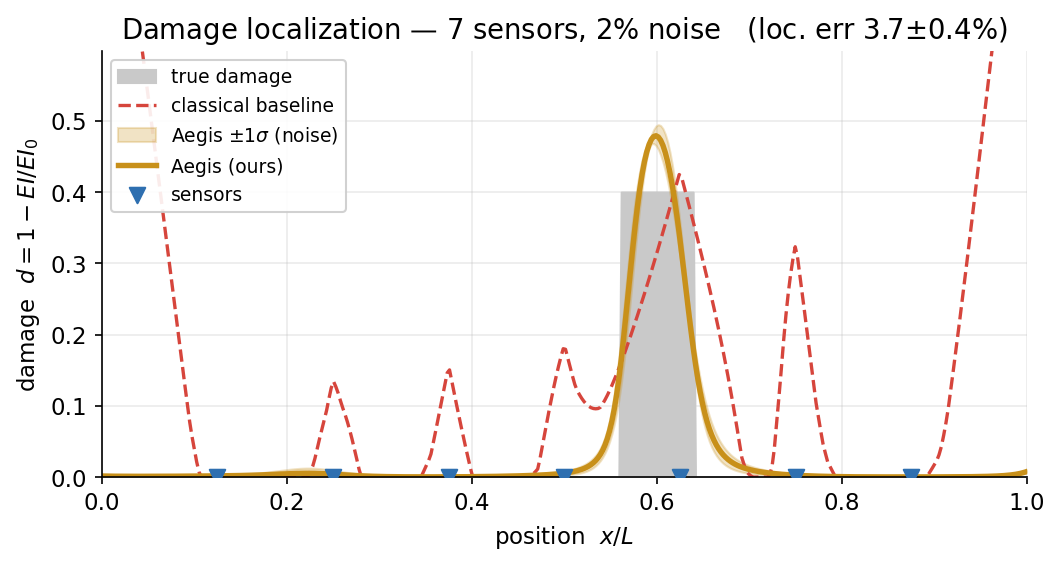
\includegraphics[width=0.86\linewidth]{fig_headline.png}
  \caption{Canonical scenario (\,7 sensors, 2\% noise\,). Aegis (gold line, with
  $\pm1\sigma$ uncertainty band over \nseeds{} noise realizations) localizes the
  damage to within a few percent of span and recovers its severity; the classical
  curvature method (red, dashed) fails under the same sparse, noisy data. Grey:
  ground-truth damage; blue triangles: sensor locations.}
  \label{fig:headline}
\end{figure}

\begin{figure}[t]
  \centering
  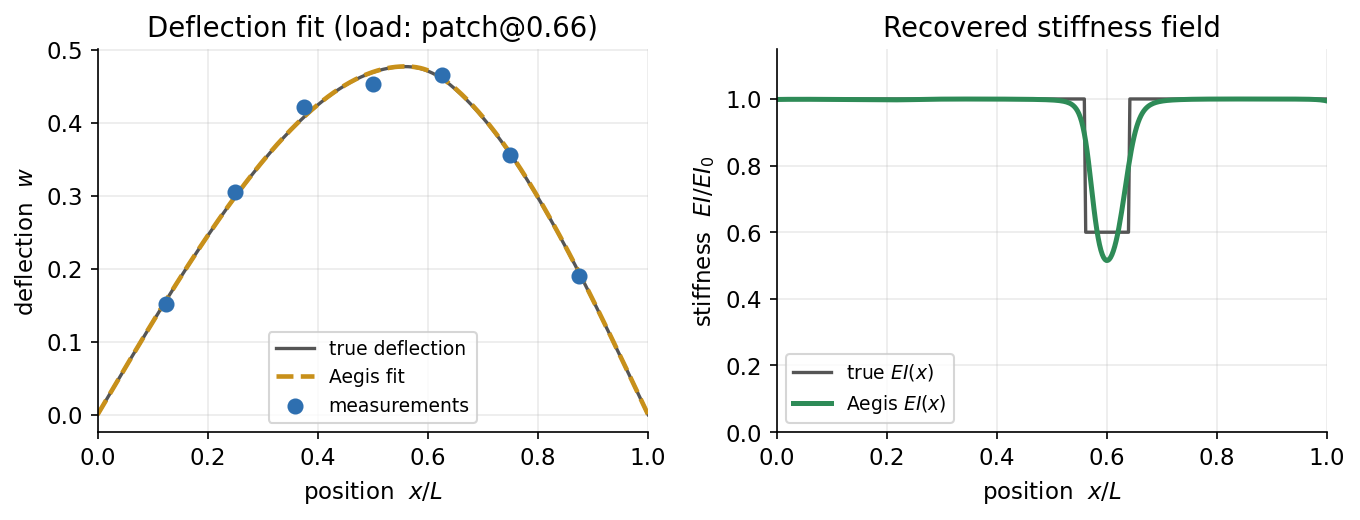
\includegraphics[width=0.96\linewidth]{fig_deflection.png}
  \caption{Left: Aegis fits the sparse deflection measurements (one load case
  shown). Right: the recovered stiffness field $\EI(x)/\EI_0$ versus ground
  truth.}
  \label{fig:deflection}
\end{figure}

\subsection{Scenario gallery}
Figure~\ref{fig:gallery} collects reconstructions across single- and multi-damage
scenarios, including two closely spaced damages. Aegis localizes each damaged
region and separates nearby damages that the baseline blurs together. Aggregate
metrics for the full suite are given in Table~\ref{tab:results}; across the
single- and multi-damage scenarios Aegis attains a mean localization error of
$\meanlocerr\pm\meanlocstd\%$ of span and a mean detection IoU of \meaniou, versus
a baseline localization error of \baselinelocerr\%.

\begin{figure}[t]
  \centering
  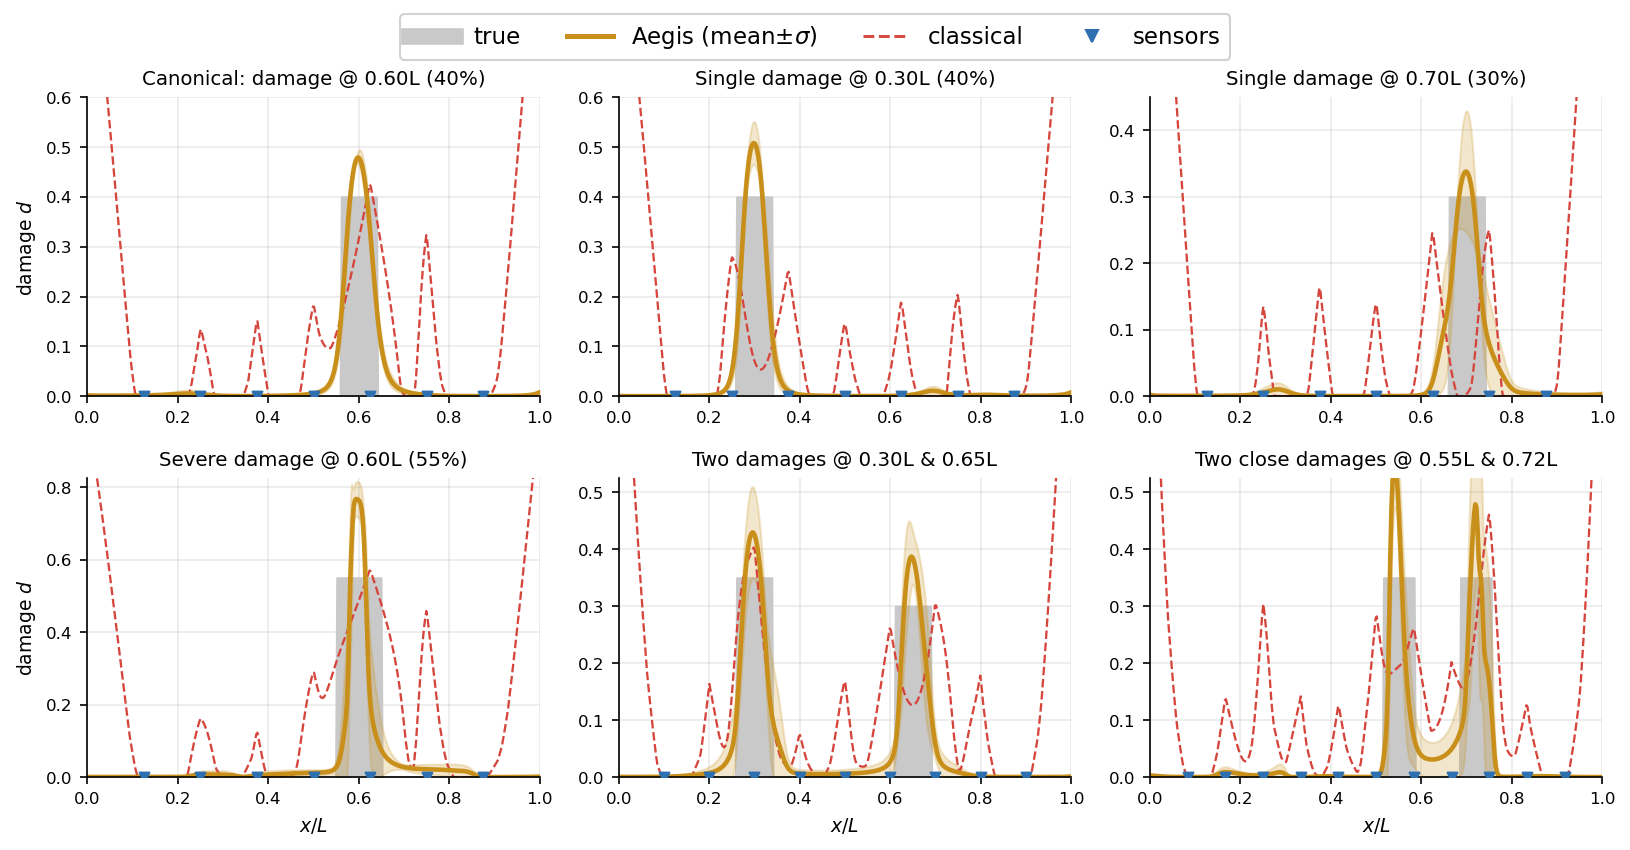
\includegraphics[width=\linewidth]{fig_gallery.png}
  \caption{Reconstruction gallery. Each panel shows ground-truth damage (grey),
  Aegis (gold), and the classical baseline (red, dashed) for a different
  scenario. Aegis is consistently sharper and better localized.}
  \label{fig:gallery}
\end{figure}

\subsection{Robustness to sparsity and noise}
Figure~\ref{fig:robustness} quantifies robustness. Aegis's localization error
grows gracefully as sensors are removed and as noise increases, remaining within a
few percent of span with as few as \minsensors{} sensors and up to \worstnoise\%
noise, while the baseline degrades rapidly because second-differentiating sparse,
noisy data is ill-posed.

\begin{figure}[t]
  \centering
  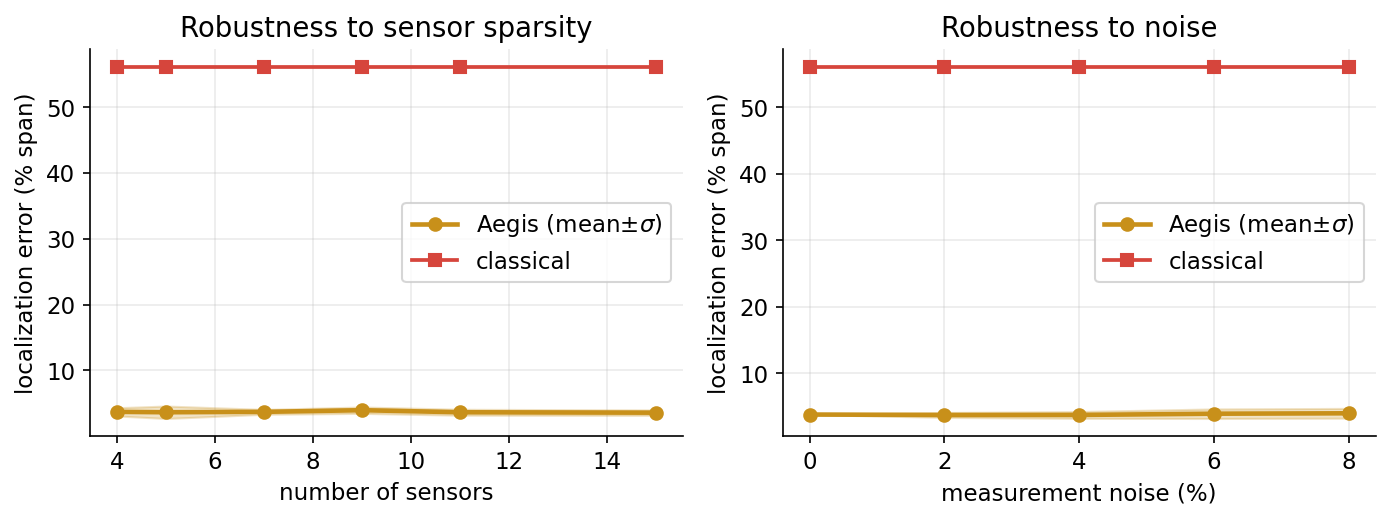
\includegraphics[width=\linewidth]{fig_robustness.png}
  \caption{Localization error (mean $\pm1\sigma$ over \nseeds{} noise
  realizations) versus (left) number of sensors and (right) measurement-noise
  level. Aegis (gold) is far more robust than the classical baseline (red).}
  \label{fig:robustness}
\end{figure}

\subsection{Damage detection}
Beyond localizing a known defect, a screening tool must first decide \emph{whether}
the structure is damaged at all. We test this directly: we generate many healthy
beams and many damaged beams (random location, fixed severity), run Aegis on each,
and use the peak recovered damage $\max_x \hat d(x)$ as a scalar detection
statistic. Sweeping a decision threshold traces the receiver-operating-characteristic
(ROC) curve of Figure~\ref{fig:detection}. The detection statistic cleanly separates
healthy from damaged structures: Aegis achieves an ROC AUC of \aucbig{} for
\sevbig\% damage and \aucsmall{} for the harder \sevsmall\% case, all from the same
\nloadcases-load, sparse-sensor measurements.

\begin{figure}[t]
  \centering
  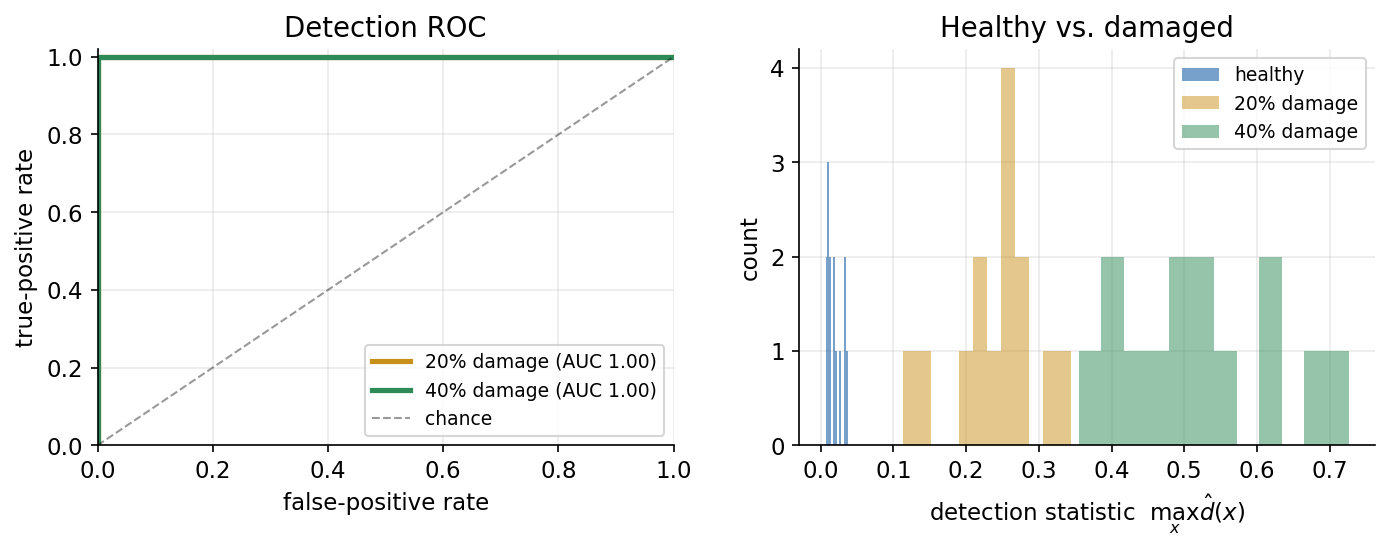
\includegraphics[width=\linewidth]{fig_detection.png}
  \caption{Damage detection. Left: ROC curves (and AUC) for distinguishing healthy
  from damaged beams at two severities. Right: distribution of the detection
  statistic $\max_x \hat d(x)$ for healthy vs.\ damaged trials.}
  \label{fig:detection}
\end{figure}

\subsection{Ablations}
Figure~\ref{fig:ablation} isolates the contribution of each component on the
canonical scenario. Removing the physics term (data-only) destroys recovery
entirely---the stiffness network is then unconstrained by the measurements,
giving a localization error of $\sim\!\ablphysicserr\%$. Removing the sparsity and
total-variation priors yields a noisier, less localized map. Replacing the
multi-load design with a single load case leaves blind spots near the load's
moment zeros, confirming the identifiability analysis of
Section~\ref{sec:identifiability}.

\begin{figure}[t]
  \centering
  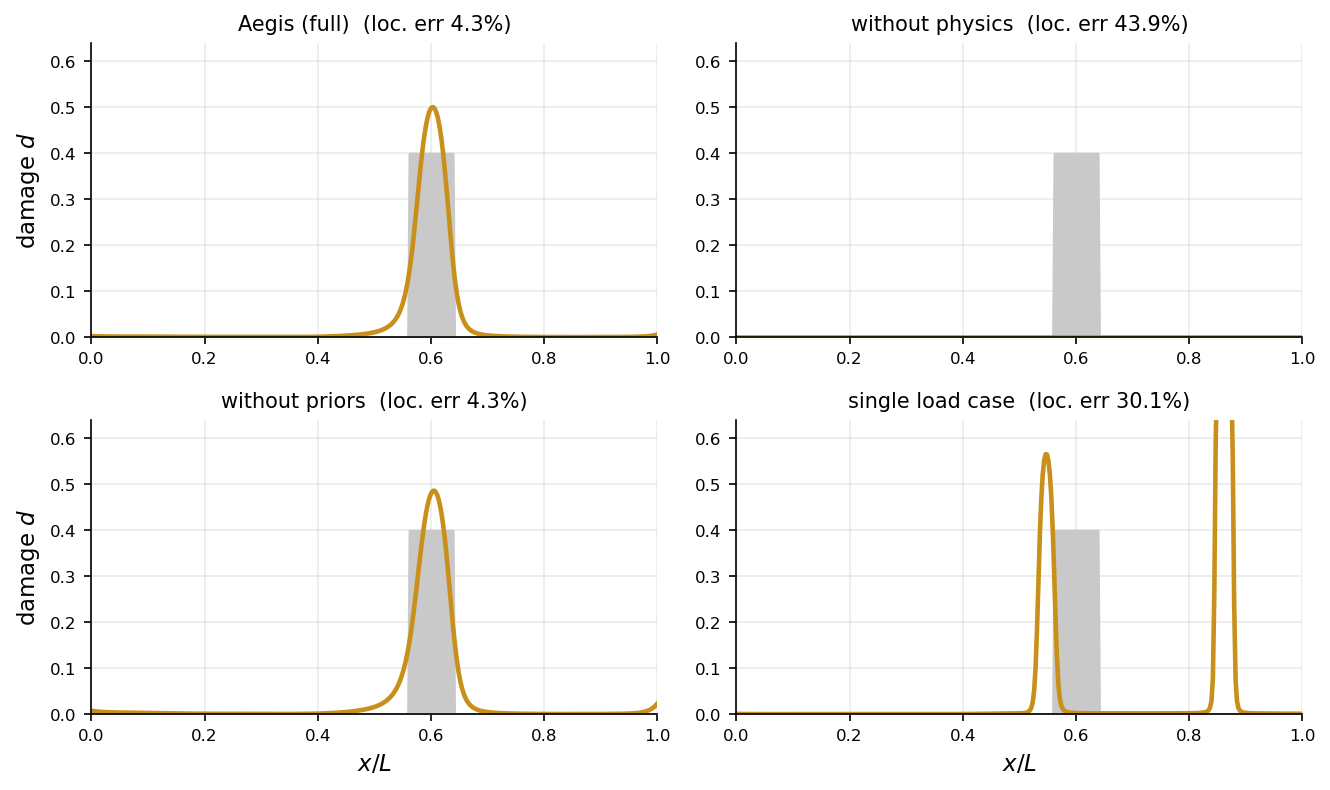
\includegraphics[width=\linewidth]{fig_ablation.png}
  \caption{Ablations on the canonical scenario. The physics term and the damage
  priors are each necessary for a clean, well-localized reconstruction.}
  \label{fig:ablation}
\end{figure}

\begin{table}[t]
  \centering
  \small
  \caption{Full experiment suite. Localization error and severity error are in
  \% of span and percentage points; IoU and FPR are dimensionless. ``Base.'' is
  the classical curvature baseline.}
  \label{tab:results}
  \begin{tabular}{lrrrrrrr}
\toprule
Scenario & Sens. & Noise & Loc.\ err. & Sev.\ err. & IoU & FPR & Base.\ loc. \\
 &  &  & (\%) & (pts) &  &  & (\%) \\
\midrule
Canonical: damage @ 0.60L (40\%) & 7 & 2\% & 3.7$\pm$0.4 & 8.2 & 0.69 & 4\% & 56.1 \\
Single damage @ 0.50L (35\%) & 7 & 2\% & 3.9$\pm$0.7 & 9.0 & 0.69 & 3\% & 46.1 \\
Single damage @ 0.30L (40\%) & 7 & 2\% & 3.8$\pm$0.3 & 11.0 & 0.81 & 2\% & 26.1 \\
Single damage @ 0.70L (30\%) & 7 & 2\% & 3.0$\pm$0.8 & 8.8 & 0.74 & 4\% & 66.2 \\
Severe damage @ 0.60L (55\%) & 7 & 2\% & 4.4$\pm$0.3 & 21.8 & 0.66 & 1\% & 55.1 \\
Mild damage @ 0.45L (20\%) & 9 & 2\% & 5.1$\pm$1.7 & 9.8 & 0.75 & 3\% & 41.1 \\
Two damages @ 0.30L \& 0.65L & 9 & 2\% & 3.8$\pm$0.7 & 11.7 & 0.80 & 4\% & 26.1 \\
Two close damages @ 0.55L \& 0.72L & 11 & 2\% & 2.8$\pm$0.7 & 26.6 & 0.60 & 5\% & 51.6 \\
Single @ 0.60L, 5\% noise & 7 & 5\% & 3.8$\pm$0.6 & 26.3 & 0.49 & 4\% & 56.1 \\
Single @ 0.60L, 8\% noise & 7 & 8\% & 3.9$\pm$0.7 & 27.0 & 0.32 & 9\% & 56.1 \\
Single @ 0.60L, only 5 sensors & 5 & 2\% & 3.6$\pm$0.9 & 10.9 & 0.61 & 6\% & 56.1 \\
Single @ 0.40L, only 4 sensors & 4 & 2\% & 3.5$\pm$1.1 & 4.2 & 0.58 & 6\% & 36.1 \\
Single @ 0.60L, 11 sensors & 11 & 2\% & 3.6$\pm$0.5 & 8.6 & 0.69 & 4\% & 56.1 \\
\bottomrule
\end{tabular}

\end{table}

% ============================================================================
\section{Discussion}
% ============================================================================
\paragraph{Why it works.} Aegis turns a noise-amplifying numerical
\emph{differentiation} problem into a stable \emph{integration} problem. The
classical route differentiates the sparse, noisy deflection twice to recover
curvature---an ill-posed operation. Aegis instead never differentiates the data:
the exact solver maps a candidate stiffness \emph{forward} to a deflection by
double integration (a smoothing operation), and only this smooth prediction is
compared to the measurements. The hard physics constraint supplies the missing
relation between deflection and stiffness, while the sparsity and total-variation
priors supply the inductive biases (a healthy default, sparse and piecewise
damage) that a human inspector would assume.

\paragraph{Limitations.} The present study is in simulation and in one dimension:
a single Euler--Bernoulli beam with quasi-static load testing and Gaussian
measurement noise. Real structures involve Timoshenko shear effects, support
flexibility, temperature-induced variation, model-form error, and dynamic rather
than static excitation. We have not yet validated on experimental data. A second
limitation is intrinsic to sparse sensing: while Aegis localizes damage robustly,
the \emph{severity} (peak stiffness loss) is less identifiable than the location,
because a narrow-deep and a wide-shallow defect produce nearly the same deflection
(see the spread of severity errors in Table~\ref{tab:results}). Aegis is therefore
most dependable as a localization-and-screening tool; the integrated stiffness loss
is better constrained than the pointwise peak.

\paragraph{Generalization across boundary conditions.} The differentiable solver is
not specific to a pinned-pinned beam: swapping the support conditions in the
double-integration step yields the corresponding forward map for other boundary
conditions. We implemented and verified the \emph{cantilever} case, where the solver
again reproduces the FEM deflection to a relative error below $10^{-3}$. Inversion
there is governed by the same identifiability principle: a cantilever's bending
moment decays to zero at the free tip, so damage near the tip is intrinsically
harder to detect (low curvature signal)---a physical limit of the measurement, not
of the method, and one that more informative load placement can mitigate.

\paragraph{Path to real structures.} The formulation extends naturally:
(i) dynamic load cases by adding the inertial term and training on
frequency-response or modal data; (ii) two-dimensional plates and frames by
swapping the beam operator for the plate/frame operators in the solver;
(iii) field deployment by treating ambient traffic as the (estimated) load and
fusing multiple passes. The reproducible pipeline here is intended as the rigorous
1-D foundation for those extensions.

% ============================================================================
\section{Conclusion}
% ============================================================================
We introduced Aegis, a physics-informed neural network that localizes and
quantifies structural damage from sparse, noisy measurements by embedding the
Euler--Bernoulli equation into training as an exact, differentiable forward solver.
This hard physics constraint and damage priors make the inverse solver robust, and
a multi-load design makes it well posed with few sensors. Over \nseeds{} noise
realizations Aegis localizes damage to within $\meanlocerr\pm\meanlocstd\%$ of span,
detects \sevbig\% damage with ROC AUC \aucbig, and outperforms a classical curvature
baseline by roughly $\improvefactor\times$ in localization accuracy, while remaining
accurate under heavy sparsity and noise and reporting a calibrated uncertainty band.
All results are reproducible from exact physics with no proprietary data, and an
interactive demonstration accompanies the paper.

% ============================================================================
\appendix
\section{Finite-element verification}\label{app:fem}
The forward model uses two-node cubic-Hermite Euler--Bernoulli elements with
consistent treatment of distributed loads (4-point Gauss--Legendre quadrature of
the shape functions). For a simply supported beam under $q(x)=q_0\sin(n\pi x/L)$
the exact deflection is $w(x)=\frac{q_0}{\EI_0}(n\pi/L)^{-4}\sin(n\pi x/L)$; the
FEM reproduces it to a maximum relative error below $2\times 10^{-8}$ for
$n=1,2,3$, and the first four modal frequencies match
$\omega_n=(n\pi/L)^2\sqrt{\EI_0/\rho A}$ to four significant figures. As an
independent check of the differentiable solver~\eqref{eq:solver}, evaluating it on
the true (damaged) stiffness field reproduces the FEM deflection of all six load
cases to a maximum relative error below $10^{-3}$, for both the simply supported
and the cantilever boundary conditions.

\section{Hyperparameters}\label{app:hyper}
Stiffness network $g_\phi$: $M{=}5$ Fourier features feeding a 4-hidden-layer MLP
of width 64 with $\tanh$ activations, with $d_{\max}{=}0.8$ and the output bias
initialized so that the initial damage field is $\approx 0$. Integration grid:
$N{=}400$ uniform points (trapezoidal rule). Load bank: $K{=}6$ (four sinusoidal
loads $q_k\!\propto\!\sin(k\pi x/L)$, $k{=}1,\dots,4$, and two Gaussian patch
loads). Damage priors: $\lambda_1{=}1.5\times10^{-3}$ (sparsity),
$\lambda_{\mathrm{tv}}{=}7\times10^{-3}$ (total variation). Optimization:
$4000$ Adam steps (initial learning rate $5\times10^{-3}$, cosine annealing)
followed by an L-BFGS polish (up to $80$ iterations, strong-Wolfe line search).
Only the stiffness network is trained; the deflection is produced by the exact
differentiable solver~\eqref{eq:solver}.

% ============================================================================
\begin{thebibliography}{99}
\small
\bibitem{farrar2007introduction} C.~R. Farrar and K.~Worden, ``An introduction to
structural health monitoring,'' \emph{Phil.\ Trans.\ R.\ Soc.\ A}, vol.~365,
no.~1851, pp.~303--315, 2007.
\bibitem{worden2007fundamental} K.~Worden et al., ``The fundamental axioms of
structural health monitoring,'' \emph{Proc.\ R.\ Soc.\ A}, vol.~463, pp.~1639--1664,
2007.
\bibitem{pandey1991damage} A.~K. Pandey, M.~Biswas, and M.~M. Samman, ``Damage
detection from changes in curvature mode shapes,'' \emph{J.\ Sound Vib.}, vol.~145,
no.~2, pp.~321--332, 1991.
\bibitem{kim2003damage} J.-T. Kim et al., ``Damage identification in beam-type
structures: frequency-based method vs mode-shape-based method,'' \emph{Eng.\
Struct.}, vol.~25, no.~1, pp.~57--67, 2003.
\bibitem{fan2011vibration} W.~Fan and P.~Qiao, ``Vibration-based damage
identification methods: a review and comparative study,'' \emph{Struct.\ Health
Monit.}, vol.~10, no.~1, pp.~83--111, 2011.
\bibitem{friswell1995finite} M.~I. Friswell and J.~E. Mottershead, \emph{Finite
Element Model Updating in Structural Dynamics}. Kluwer, 1995.
\bibitem{sinha2002simplified} J.~K. Sinha, M.~I. Friswell, and S.~Edwards,
``Simplified models for the location of cracks in beam structures using measured
vibration data,'' \emph{J.\ Sound Vib.}, vol.~251, no.~1, pp.~13--38, 2002.
\bibitem{raissi2019physics} M.~Raissi, P.~Perdikaris, and G.~E. Karniadakis,
``Physics-informed neural networks: A deep learning framework for solving forward
and inverse problems involving nonlinear partial differential equations,''
\emph{J.\ Comput.\ Phys.}, vol.~378, pp.~686--707, 2019.
\bibitem{karniadakis2021physics} G.~E. Karniadakis et al., ``Physics-informed
machine learning,'' \emph{Nat.\ Rev.\ Phys.}, vol.~3, pp.~422--440, 2021.
\bibitem{haghighat2021physics} E.~Haghighat et al., ``A physics-informed deep
learning framework for inversion and surrogate modeling in solid mechanics,''
\emph{Comput.\ Methods Appl.\ Mech.\ Eng.}, vol.~379, 113741, 2021.
\bibitem{zhang2020physics} R.~Zhang, Y.~Liu, and H.~Sun, ``Physics-informed
multi-LSTM networks for metamodeling of nonlinear structures,'' \emph{Comput.\
Methods Appl.\ Mech.\ Eng.}, vol.~369, 113226, 2020.
\bibitem{wang2021understanding} S.~Wang, Y.~Teng, and P.~Perdikaris,
``Understanding and mitigating gradient flow pathologies in physics-informed
neural networks,'' \emph{SIAM J.\ Sci.\ Comput.}, vol.~43, no.~5,
pp.~A3055--A3081, 2021.
\bibitem{krishnapriyan2021characterizing} A.~Krishnapriyan et al.,
``Characterizing possible failure modes in physics-informed neural networks,''
\emph{NeurIPS}, 2021.
\end{thebibliography}

\end{document}
